\documentclass{article}

% NeurIPS style: put neurips_2026.sty next to this file (Overleaf's NeurIPS template, or the NeurIPS site).
% nonatbib: NeurIPS loads natbib by default, which clashes with biblatex.
\usepackage[preprint,nonatbib]{neurips_2026}

\usepackage[utf8]{inputenc}
\usepackage[T1]{fontenc}
\usepackage{hyperref}
\usepackage{url}
\usepackage{booktabs}
\usepackage{amsfonts,amsmath}
\usepackage{microtype}
\usepackage{xcolor}
\usepackage{graphicx}
\usepackage{pgfplots}
\pgfplotsset{compat=1.17}
\usepackage[style=alphabetic,maxbibnames=99]{biblatex}
\addbibresource{references.bib}

\title{Adaptive Test-Time Training Budgets for ARC-AGI\\[2pt]\large Midway Report}

\author{%
  Avi Karthikeyan \\ \texttt{avijithk@andrew.cmu.edu} \And
  \textcolor{red}{[Partner name]} \\ \texttt{\textcolor{red}{[andrewid]}@andrew.cmu.edu}
}

\begin{document}
\maketitle

% ---------------------------------------------------------------------------
\section{Introduction}

The Abstraction and Reasoning Corpus (ARC-AGI-1) \cite{chollet2019measure} tests few-shot rule induction: each task gives 2--10 demonstration pairs of colored grids (up to $30\times30$, 10 colors) and asks for the output of a new input grid. Every evaluation task uses a rule unseen in training, so memorization does not help; this makes ARC a direct probe of how deep models generalize from a handful of examples. We use the 400 training tasks for fine-tuning and report on the 400 public evaluation tasks.

We serialize grids as text (one digit per cell, one line per row) and model the task with a pretrained decoder-only language model, Qwen2.5-0.5B \cite{qwen2024qwen25}, adapted with LoRA \cite{hu2021lora}. An LLM suits the task because the prompt can hold the demonstrations in context, and LoRA keeps per-task adaptation cheap. On top of this baseline we use \emph{test-time training} (TTT): a fresh adapter is trained on each test task's own demonstrations before predicting. Our contribution targets the cost of TTT: we study \emph{adaptive} per-task budgets that stop training once a task appears learned. We evaluate with the official ARC score (exact match with any of 2 attempts), plus cell accuracy and output-size match of the first attempt, and GPU-seconds per task.

% ---------------------------------------------------------------------------
\section{Literature review}

\textbf{\textcite{chollet2019measure}} defines intelligence as skill-acquisition efficiency and introduces ARC to measure it, with tasks built on core-knowledge priors (objects, counting, geometry) and held-out evaluation rules. It sets the problem and the metric we use.

\textbf{\textcite{akyurek2024surprising}} show that test-time training makes LMs far stronger on ARC: per task, they build leave-one-out training examples from the demonstrations, expand them with invertible augmentations, and fine-tune a LoRA adapter before predicting with augmentation voting. This gave up to $6\times$ higher accuracy than the fine-tuned model alone and 53\% on the public validation set with an 8B model. Its novelty is treating each test task as a tiny training set rather than relying on in-context learning alone. Our TTT pipeline follows their recipe; they use one fixed budget for every task.

\textbf{\textcite{franzen2025product}} reach 71.6\% on the public evaluation set at about 2 cents per task. Their key idea is a \emph{product of experts} (PoE): each candidate answer is re-scored by the model's probability under several augmented views of the task, and those probabilities are multiplied. This works better than majority voting because a wrong answer is rarely likely under every view. We adopt PoE as a component and cite it as prior work.

\textbf{\textcite{deliege2026trainingbudgets}} run a controlled study of pretraining and TTT budgets for two ARC models (VARC and TRM) and find that the per-task TTT budget strongly affects accuracy while dominating total compute. All of these works spend the \emph{same} budget on every task; we ask whether budgets can be set per task.

% ---------------------------------------------------------------------------
\section{Methods}

\textbf{Data and augmentation.} A grid becomes digit rows; a prompt lists the demonstrations (\texttt{Input:} and \texttt{Output:} blocks) and ends with the test input. Qwen's tokenizer splits digits individually, so a $30\times30$ grid costs about 930 tokens; 99\% of training prompts fit in 8,192 tokens, and longer ones drop demonstrations from the front. Augmentations are the 8 dihedral symmetries combined with random permutations of colors 1--9 (background 0 fixed); all are invertible, so predictions are mapped back to the original frame.

\textbf{Baseline.} We fine-tune Qwen2.5-0.5B (base) with LoRA (rank 32, $\alpha=64$, all attention and MLP projections; 17.6M trainable parameters, 3.4\%). Each sample picks one pair of a training task as the query and the others as demonstrations, under a random augmentation; 8 samples per task per epoch, 2 epochs, effective batch 16, AdamW at $2\times10^{-4}$ with cosine decay. Loss is computed only on the output grid and end token. Training took 34 minutes on one NVIDIA A10G (AWS g5.xlarge). Prediction is greedy, with a second attempt on the transposed task.

\textbf{Test-time training.} Starting from the baseline (adapter merged), each evaluation task gets a fresh rank-32 LoRA adapter, reset to the same initialization. Its training set is the leave-one-out examples of the task's demonstrations under 16 augmentations; it trains at a constant learning rate of $10^{-4}$, batch 1. We log predictions at steps $\{0, 8, 16, 32, 64\}$, so one run yields every fixed budget, and log the mean leave-one-out loss every 4 steps as a candidate stopping signal. Each prediction greedily decodes one candidate under each of 8 augmentations, then picks two answers by \emph{voting} (most frequent) or \emph{PoE} (highest summed log-probability across the 8 views, over the top-8 candidates). Step 0 is the baseline with augmentation ensembling and no TTT.

\textbf{Adaptive stopping (offline).} Because every checkpoint is logged, we replay stopping rules per task: walk the checkpoints and stop at the first where the rule fires, charging training time up to that point plus one prediction. We test thresholds on the leave-one-out loss and a plateau rule (stop when the loss falls by less than $\delta$ since the previous checkpoint).

% ---------------------------------------------------------------------------
\section{Preliminary results}

\begin{table}[h]
\centering
\caption{ARC-AGI-1 public evaluation (400 tasks), Qwen2.5-0.5B. Cell accuracy and size match use the first attempt; seconds are GPU time per task on one A10G (training to that step + one prediction).}
\label{tab:main}
\small
\begin{tabular}{lcccc}
\toprule
Method & ARC score & Cell acc. & Size match & s / task \\
\midrule
Baseline, direct (2 attempts) & 3.1\% & 45.5\% & 60.5\% & 15.1 \\
Baseline + 8 views, vote / PoE & 3.1 / 4.5\% & 52.0 / 60.2\% & 68.0 / 77.9\% & 19.3 / 23.7 \\
TTT 16 steps, vote / PoE & 10.0 / 10.9\% & 49.8 / 61.1\% & 62.4 / 75.5\% & 25.1 / 29.2 \\
TTT 32 steps, vote / PoE & 12.4 / 15.5\% & 55.8 / 64.4\% & 68.1 / 77.1\% & 28.0 / 32.7 \\
TTT 64 steps, vote / PoE & 13.4 / \textbf{16.6\%} & 54.0 / 65.8\% & 65.5 / 77.9\% & 37.0 / 42.1 \\
Adaptive: loss plateau $<5\%$, vote / PoE & 13.8 / 16.3\% & -- & -- & 34.3 / 39.1 \\
\bottomrule
\end{tabular}
\end{table}

\begin{figure}[h]
\centering
\begin{minipage}{0.49\linewidth}
\centering
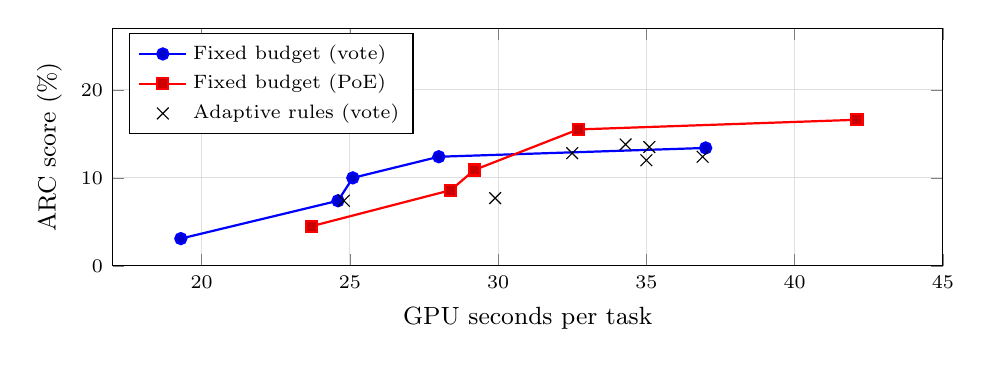
\begin{tikzpicture}
\begin{axis}[width=\linewidth, height=4.6cm, ymin=0, ymax=27, xmin=17, xmax=45, xlabel={GPU seconds per task}, ylabel={ARC score (\%)},
  legend style={font=\scriptsize, at={(0.02,0.98)}, anchor=north west}, legend cell align=left, tick label style={font=\scriptsize},
  label style={font=\small}, grid=major, grid style={gray!25}]
\addplot+[mark=*, thick] coordinates {(19.3,3.1) (24.6,7.4) (25.1,10.0) (28.0,12.4) (37.0,13.4)};
\addplot+[mark=square*, thick] coordinates {(23.7,4.5) (28.4,8.6) (29.2,10.9) (32.7,15.5) (42.1,16.6)};
\addplot+[only marks, mark=x, mark size=3pt, black] coordinates {(36.9,12.4) (35.0,12.0) (29.9,7.7) (24.8,7.4) (35.1,13.5) (34.3,13.8) (32.5,12.8)};
\legend{{Fixed budget (vote)},{Fixed budget (PoE)},{Adaptive rules (vote)}}
\end{axis}
\end{tikzpicture}
\end{minipage}\hfill
\begin{minipage}{0.49\linewidth}
\centering
\IfFileExists{figs/loss.png}{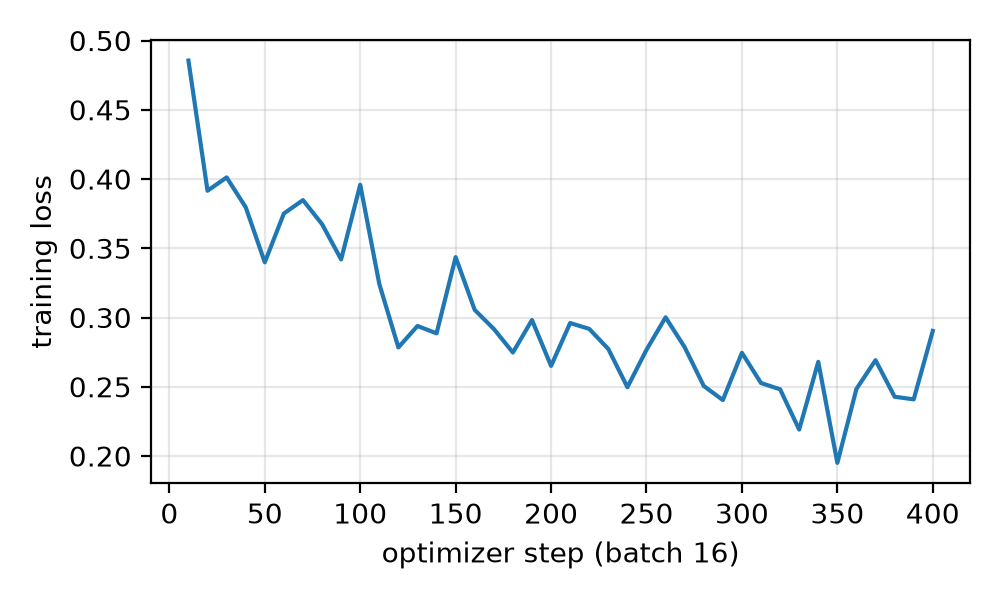
\includegraphics[width=\linewidth]{figs/loss.png}}{\fbox{\parbox{0.9\linewidth}{\centering\vspace{1.5cm}copy \texttt{loss.png} to \texttt{figs/}\vspace{1.5cm}}}}
\end{minipage}
\caption{Left: accuracy vs.\ compute; fixed budgets are steps 0, 8, 16, 32, 64. Right: baseline training loss (0.49 $\rightarrow$ 0.25 over 400 steps).}
\label{fig:curves}
\end{figure}

TTT raises the ARC score from 3.1\% (baseline) to 16.6\% (64 steps, PoE), a $5.3\times$ gain. PoE beats voting at every budget, by 1.1--3.1 points. The leave-one-out loss predicts which tasks are solved, increasingly so with training: AUC 0.58 at step 0, 0.71 at step 16, 0.76 at step 64.

% ---------------------------------------------------------------------------
\section{Evaluation of preliminary work}

\textbf{What worked.} TTT gives the large gains reported in the literature even at 0.5B parameters, and PoE adds a consistent margin over voting, matching \textcite{franzen2025product}. Accuracy still rises from 32 to 64 steps, but by only about one point, so returns are diminishing.

\textbf{What did not.} We hoped some stopping rule would match the 64-step score with clearly less compute. Absolute loss thresholds do worse than simply using a smaller fixed budget: stopping at the median loss uses 82\% of the compute but scores 10.6\% (PoE), below fixed 32 steps (15.5\% at 78\%). We think absolute losses are not comparable across tasks: large, copy-heavy outputs have low per-token loss even when wrong. The plateau rule matches the 64-step score with about 7\% less compute, close to break-even. Two further limits appeared. First, one prediction costs about as much as 64 training steps ($\sim$20\,s each), so adapting only the training budget can save at most about 43\% of per-task cost. Second, cell accuracy and size match briefly \emph{drop} at step 8 before recovering, suggesting early TTT disrupts the model. The baseline alone is weak (3.1\%): some direct predictions run to the output length cap without producing a valid grid.

% ---------------------------------------------------------------------------
\section{Future work}

We will make the whole pipeline adaptive and strengthen the base model. (1) \emph{Better stopping signals}: a truly held-out demonstration, and losses measured relative to each task's own starting value rather than absolute thresholds. (2) \emph{Adaptive inference}: generate candidates in small batches and stop once they agree, since prediction is half the cost; this is our main original component. (3) \emph{Stronger baseline}: fine-tune on procedurally generated training tasks (re-arc \cite{hodel2024rearc}) and test whether a stronger model needs fewer TTT steps, and compare Qwen2.5-1.5B. (4) Ablations (LoRA rank, attention vs.\ MLP adapters, augmentations) and a transfer check on ConceptARC. We will evaluate the final method by its accuracy--compute curve on all 400 tasks against fixed budgets, and confirm the savings in a real (not replayed) adaptive run.

% ---------------------------------------------------------------------------
\section{Timeline and division of labor}

\textbf{A} (\textcolor{red}{[name]}): data, baseline, re-arc pipeline, ablations, ConceptARC. \textbf{B} (\textcolor{red}{[name]}): TTT, adaptive inference, stopping rules, online adaptive run. \textbf{Nov 11--15}: build re-arc and adaptive inference; held-out signal run. \textbf{Nov 15--22}: re-arc TTT on all 400 tasks, adaptive inference, 1.5B, ablations, ConceptARC. \textbf{Nov 24}: Check-in 2. \textbf{Nov 25--28}: real adaptive run and reruns. \textbf{Nov 29--Dec 2}: final report. Compute: about 50 more GPU-hours on two AWS accounts.

\printbibliography

\end{document}
